\documentclass[conference]{IEEEtran}
\IEEEoverridecommandlockouts
% The preceding line is only needed to identify funding in the first footnote. If that is unneeded, please comment it out.
\ifCLASSOPTIONcompsoc
 \usepackage[caption=false, font=normalsize, labelfont=sf, textfont=sf]{subfig}
\else
 \usepackage[caption=false, font=footnotesize]{subfig}
\fi
\usepackage{cite}
\usepackage{amsmath,amssymb,amsfonts}
\usepackage{hyperref}
\usepackage{algorithmic}
\usepackage{graphicx}
\usepackage{textcomp}
\usepackage{xcolor}
\usepackage{url}
\usepackage{soul}
\def\BibTeX{{\rm B\kern-.05em{\sc i\kern-.025em b}\kern-.08em
    T\kern-.1667em\lower.7ex\hbox{E}\kern-.125emX}}
\begin{document}

\title{Provenance--aware workflow for data quality management and
	improvement for large continuous scientific data streams\\
}
%% co-authors in alphabetical order
\author{\IEEEauthorblockN{Jitendra Kumar\IEEEauthorrefmark{1},
	                      Ranjeet Devarakonda\IEEEauthorrefmark{1},
	                      Michael Giansiracusa\IEEEauthorrefmark{1},
	                      Kavya Guntupally\IEEEauthorrefmark{1},
	                      Joseph V. Olatt\IEEEauthorrefmark{2}, \\
	                      Zach Price\IEEEauthorrefmark{2},
	                      Alka Singh\IEEEauthorrefmark{3},
	                      Harold A. Shanafield III\IEEEauthorrefmark{1}
}\\
\IEEEauthorblockA{\IEEEauthorrefmark{1}Environmental Sciences Division, 
Oak Ridge National Laboratory, Oak Ridge, TN, USA \\
Email: jkumar@climatemodeling.org, 
	   devarakondar@ornl.gov, 
       giansiracumt@ornl.gov,\\
       guntupallyk@ornl.gov, 
       shanafieldha@ornl.gov}
\IEEEauthorblockA{\IEEEauthorrefmark{2}Information Technology
	Services Division, 
Oak Ridge National Laboratory, Oak Ridge, TN, USA \\
Email: olattjv@ornl.gov, pricezt@ornl.gov}

\IEEEauthorblockA{\IEEEauthorrefmark{3}Electrical and
	Electronics Systems Research Division, 
Oak Ridge National Laboratory, Oak Ridge, TN, USA \\
Email: singhar@ornl.gov}
}
\maketitle
%% Abstract
\begin{abstract}
Data quality assessment, management and improvement is an integral part of
any big data intensive scientific research to ensure accurate, reliable, and
reproducible scientific discoveries. The task of maintaining the quality of
data, however, is non-trivial and poses a challenge for a program like
the Department of Energy's Atmospheric Radiation Measurement (ARM) that
collects data from hundreds of instruments across the world, and
distributes thousands of streaming data products that are continuously
produced in near-real-time for an archive 1.7 Petabyte in size and
growing. In this paper, we present a computational data processing
workflow to address
the data quality issues via an easy and intuitive web-based portal that
allows reporting of any quality issues for any site, facility or
instruments at a granularity down to individual variables in the data
files. This portal allows instrument specialists and scientists to provide
corrective actions in the form of symbolic equations. A parallel processing
framework applies the data improvement to a large volume of data in an
efficient, parallel environment, while optimizing data transfer and file
I/O operations; corrected files are then systematically versioned and
archived. A provenance tracking module tracks and records any change
made to the data during its entire life cycle which are communicated
transparently to the scientific users. Developed in Python using open
source technologies, this software architecture enables fast and efficient
management and improvement of data in an operational data center
environment. 
\end{abstract}




\begin{IEEEkeywords}
scientific data workflows, data quality, provenance, atmospheric science, 
\end{IEEEkeywords}


%% Introduction
\section{INtroduction}


%% ARM intro 
\section{Atmospheric Radiation Measurement}
\subsection{Introduction to ARM program}
For 30 years and counting since its inception in 1990
\cite{Turner_AMS_2016}, ARM program has
been collecting observations across the globe to advance the robust
predictive understanding of Earth's climate and environmental systems
and to inform the development of sustainable solutions to the Nation's
energy and environmental challenges. Deployed across three atmospheric
observatories, three mobile facilities and aerial facilities, data are
continuously being collected from 480 scientific instruments and
sensors. With 1.7 Petabyte and growing archive of data, ARM makes
available to the scientific community, publicly and freely,
approximately 8218 data streams of which 1220 are actively growing in
near-real-time with data streaming from the instruments around the
world.

\begin{figure*}
 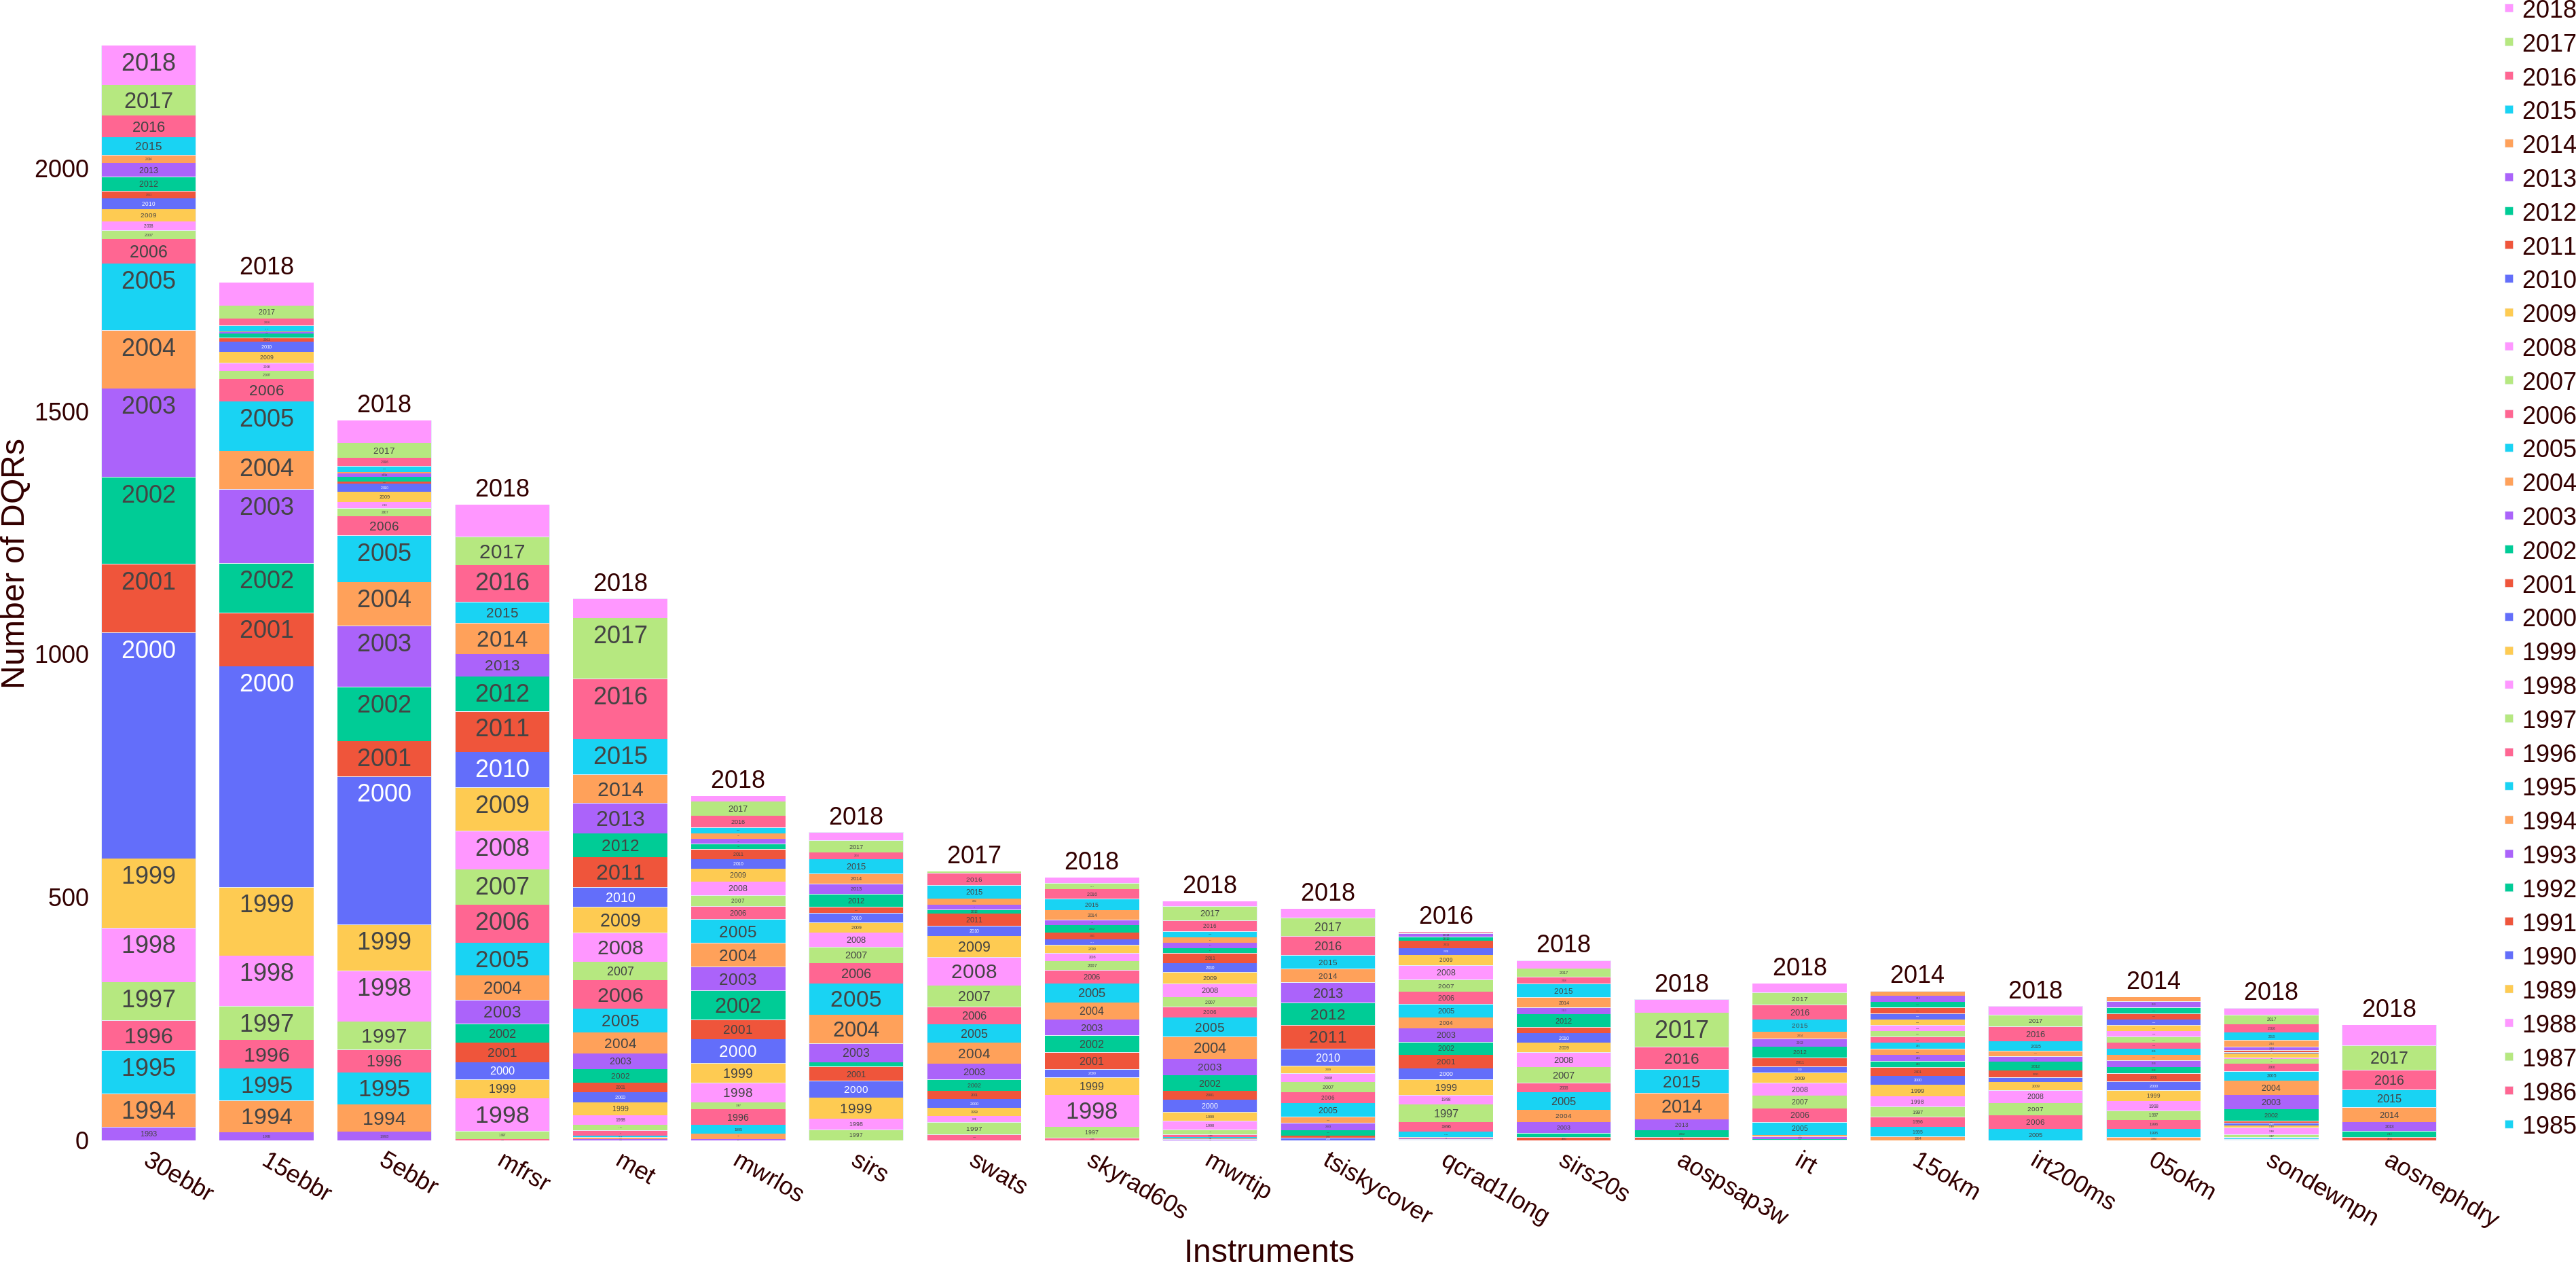
\includegraphics[width=\linewidth]{figures/dqr_by_instrument_20.png}
 \caption{DQRs for select 20 instruments over the period 1993-2019 show
 that some instruments are more prone to data quality issues than
 the others. Time series of DQRs show that data quality issues at many
 of the instruments are repetitive and recurring.}
 \label{fig:dqr_by_instrument}
\end{figure*}


\subsection{Assessment and Management of Data Quality}
These instruments for atmospheric observations, however, are prone to data quality issues due to
the challenging operating conditions in field
%(Figure~\ref{fig:dqr_by_instrument})
, sensor failures, need for
re-calibration etc. ARM Data Quality Office, established in year 2000,
coordinates detection and reporting of data quality for all data streams
\cite{Peppler_AMS_2016,peppler2005,peppler2008quality}.


Data Quality Reports (DQR) can be submitted by data quality analysts,
instrument mentors, facilities operations personnel or data users and
are saved within a consistent and searchable PostgreSQL database.
However, with large numbers of instruments and streaming data stream
maintained by the program, DQRs can be frequent and many. 
Figure~\ref{fig:dqr_by_instrument} shows the reported data quality
issues for 20 ARM instruments over time. Some instruments are more prone
to data quality issues than, often due to the nature of deployed
sensors, and its essential that the data be reprocessed to ensure the
availability of high quality continuous time series. Within ARM program,
reprocessing of data is conducted whenever a data quality issue that can
be corrected is identified. Reprocessing is also conducted if an
improved processing algorithm is available. However, the volume and
diversity of data poses a challenge.

Historically the complexity of data reprocessing to address the quality
issues, data size and volume has limited the improvements made to
correct for the data quality issue
(Figure~\ref{fig:dqr_instrument_per_year}). For example, 30 minute
resolution energy balance Bowen Ratio (30EBBR)
instruments that have been in operation since 1993 has largest number of
DQRs, most of which have not been addressed. Surface meteorology (MET)
observations, which are one of highly used datasets, had large number of
reported quality issues, only few of which has been corrected. In
contrast, radiation measurements (RAD) instruments had very few quality
issues, most of which were collected. 

\begin{figure}
 \centering
 \subfloat[30 minute Energy Balance Bowen Ratio (EBBR) instruments are
 one of the longest running core instruments within ARM and while it had
 a number of reported data quality issues every year, most of them have
 not been addressed.]{
  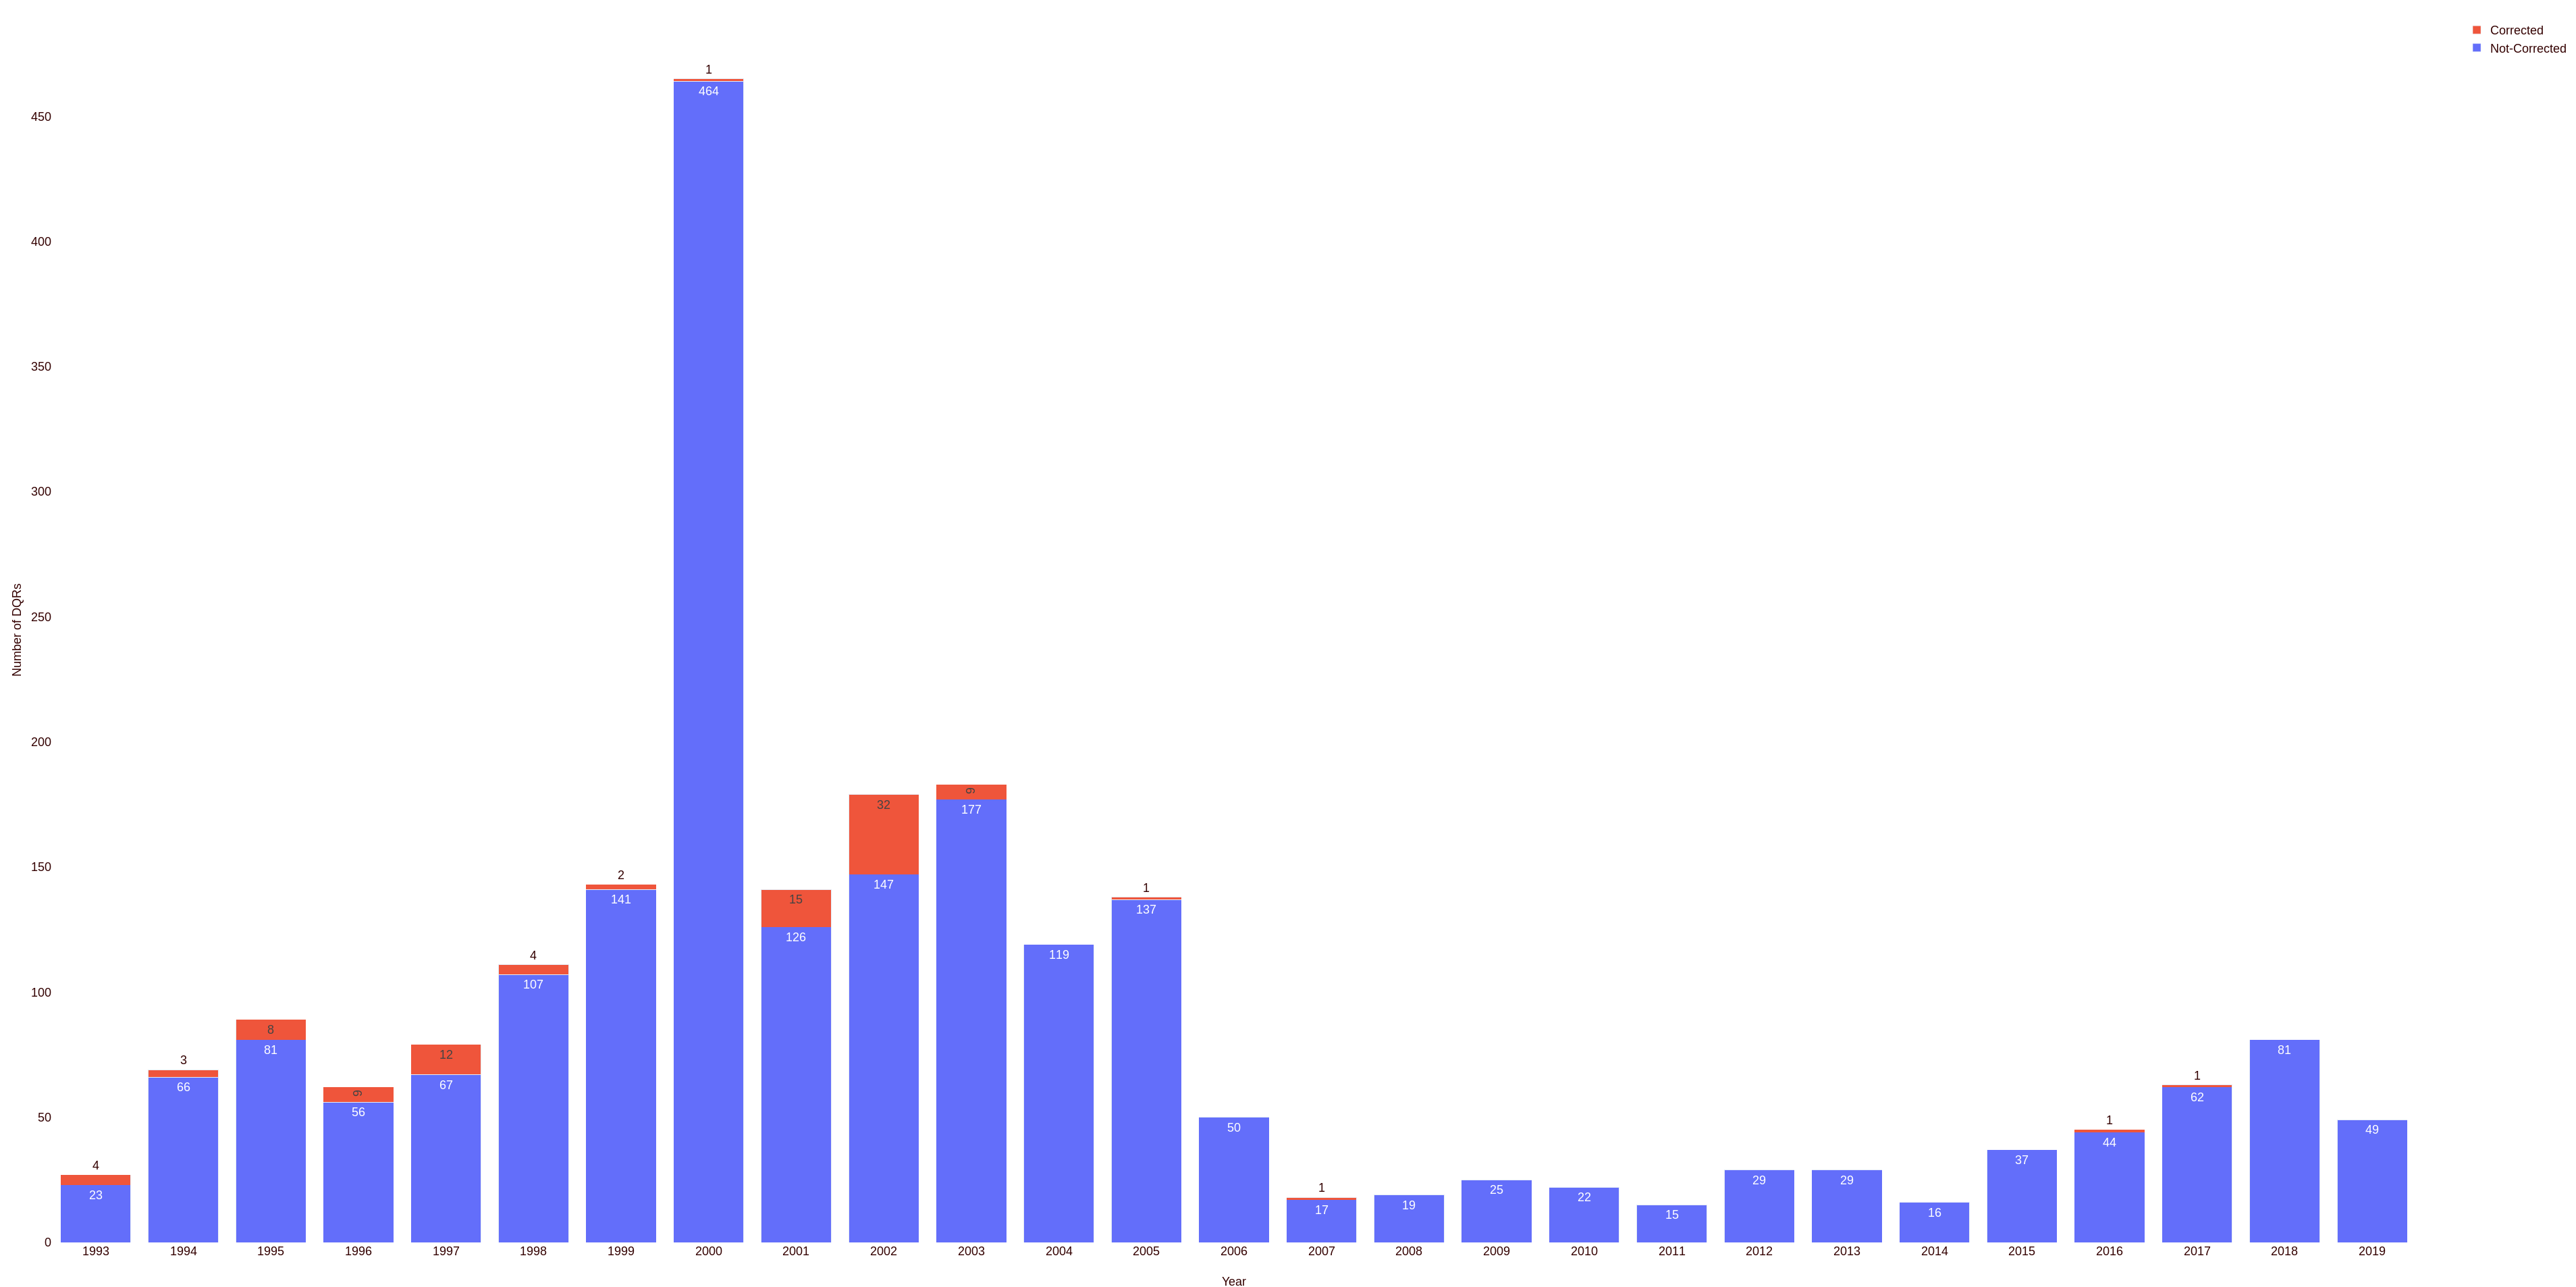
\includegraphics[width=\linewidth]{figures/30ebbr_dqr_reproc_by_year.png}
 }\\
 \subfloat[Surface Meteorology (MET) are another core instruments at ARM
 facilities that with frequent reported data quality issues, and
 many of them have been addressed in recent years as data quality
 improvement infrastructure has improved.]{
  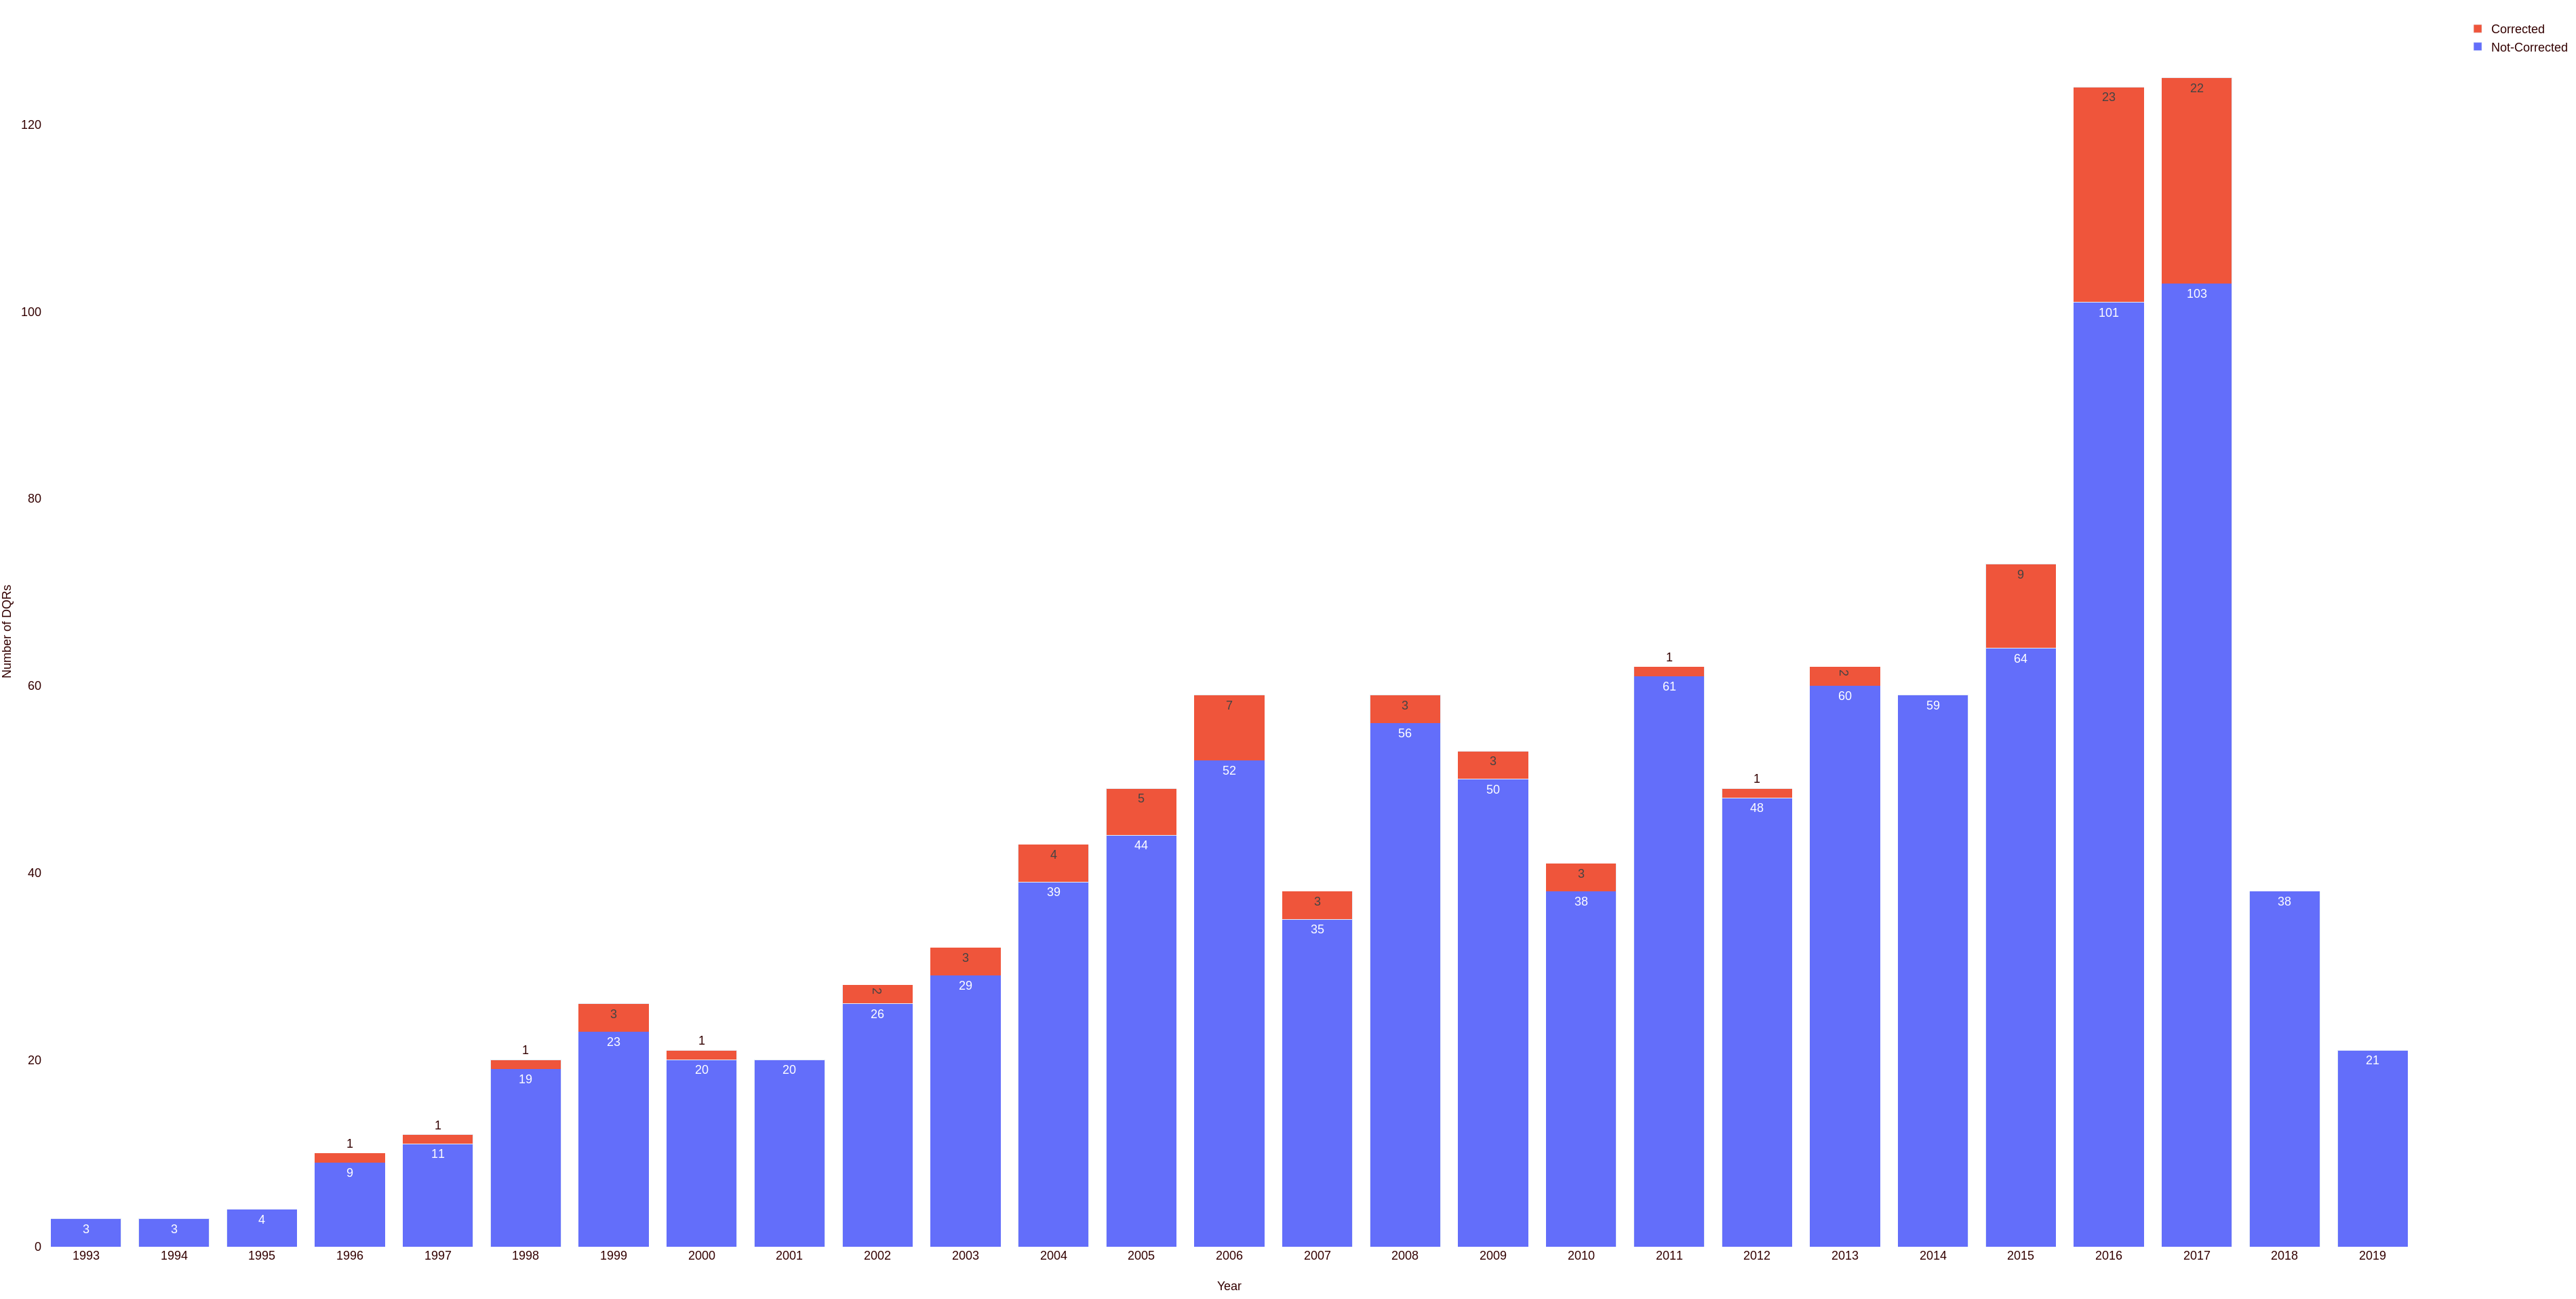
\includegraphics[width=\linewidth]{figures/met_dqr_reproc_by_year.png}
 }\\
 \subfloat[Radiation Measurements (RAD) instruments have had fairly
 small number of data quality issues, most of which have been addressed.]{
  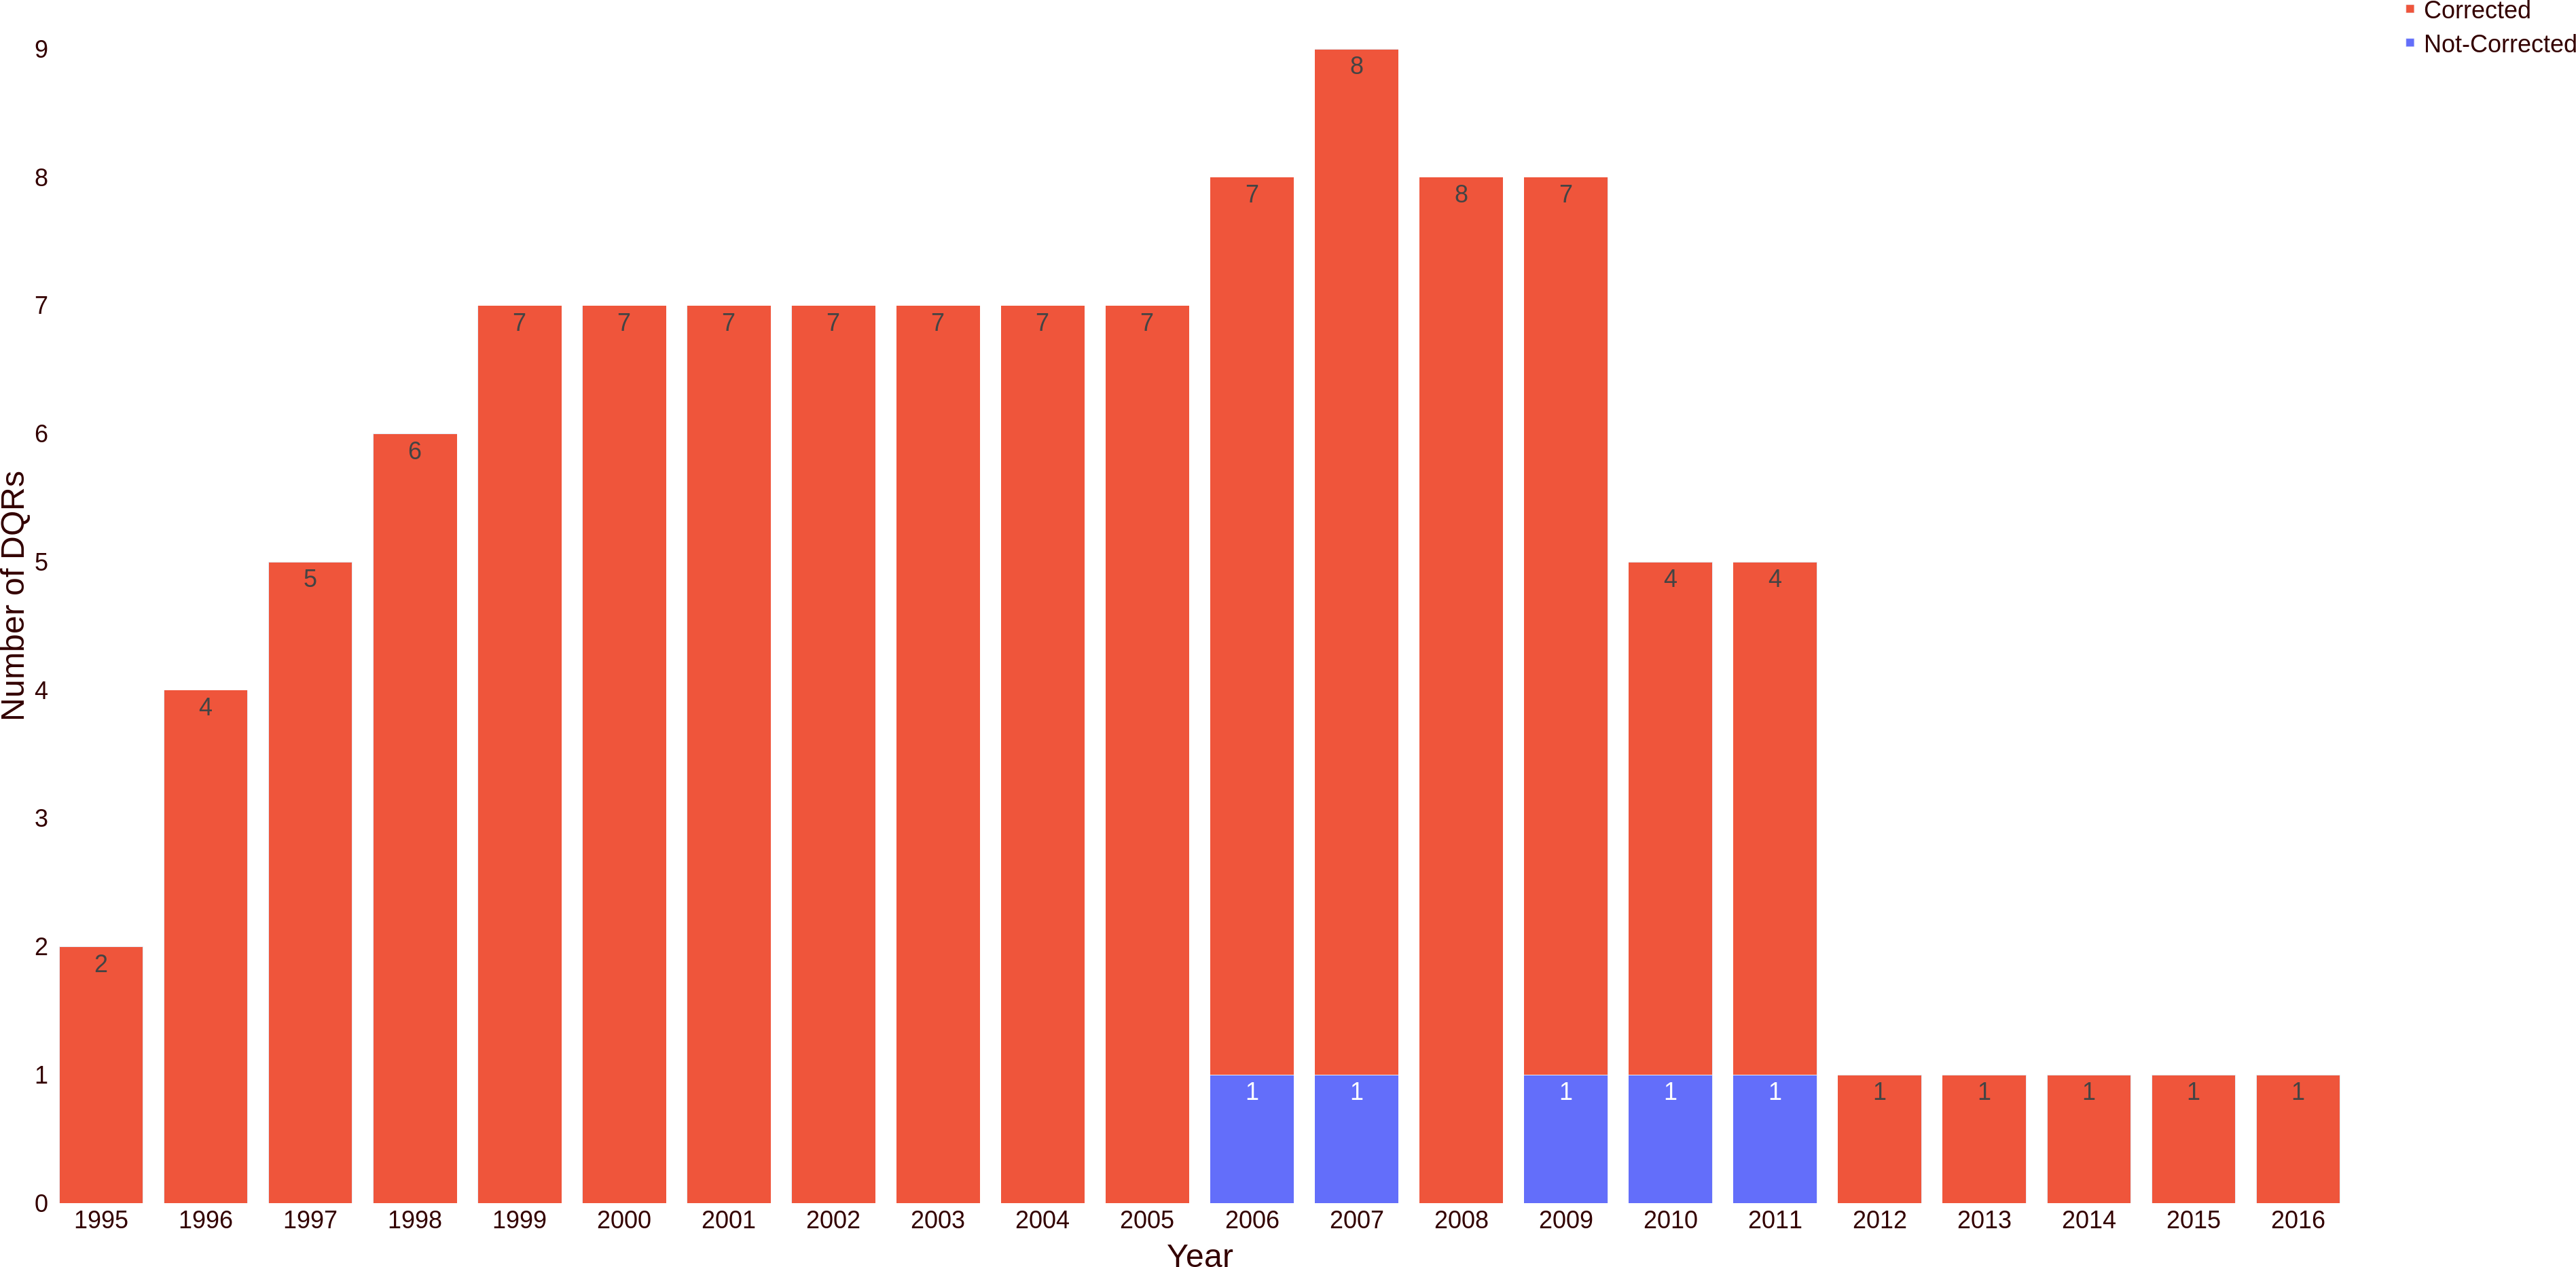
\includegraphics[width=\linewidth]{figures/radflux_dqr_reproc_by_year.png}
 }
 \caption{Only a small fraction of reported quality issues are corrected
 (shown in red) while majority remains uncorrected (shown in blue).
	 Fraction of corrected vs not-corrected are highly variable across
	 different instruments and are often determined by availability of
	 resolution for the issue, process complexity and data volume.}
 \label{fig:dqr_instrument_per_year}
\end{figure}


%% Objectives
\section{Objectives}
Objective of our study was to develop an efficient computational
workflow for processing atmospheric science data sets to address data
quality issues. Workflow was designed to 1) allow for easy and intuitive
data quality issue reporting system to encourage data correction in
addition to reporting; 2) automation of data reprocessing to reduce
human intervention and thus maximizing efficiency; 3) parallel
processing of large data volumes; 4) systematic process verification and
version control; 5) capture provenance information at each step; and 6)
clearly communication to all stakeholders about any update to the data.



%% Reprocessing workflow
\section{Workflow for data quality improvement}
A computational workflow for reprocessing data to address data quality
issue was developed in Python programming language. The software
framework was designed for computational performance and cross-platform
compatibility.

\subsection{Data Quality Reporting Tool}



\subsection{Automating data processing}

\subsubsection{Instrument data dictionaries}

\subsubsection{Data staging and processing environment}

\subsubsection{Symbolic equations processing}

\subsubsection{Data review}


\section{Data versioning and archival}
Once an updated version of data with improved data quality is prepared,
it is formally assigned a version for tracking. However, versioning for
complex data like those in ARM pose unique challenges which led to
development of new data versioning system deployed across the facility
\cite{Macduff_2014}. Data reprocessing to data quality improvement,
however, at times leads to versioning conflict scenarios. Versioning
module of the workflow extends the current versioning scheme
\cite{Macduff_2014}.

Standard ARM filename and versioning includes site, facility, instrument
and start time of observation time series in filename. However, length
of time series contained within the file are not reflected in the
filename and thus creating conflict when data are reprocessed.
ARM file standards also allow for any arbitrary number of files within a day
during a real time processing, while reprocessing for data quality
improvements on past data often create longer continuous time series and
thus few files. To identify and address these conflicts all affected
files (old and new) were checked for the start and end of the time
series. In particular following scenarios occur frequently: 

\begin{enumerate}
 \item Near-real-time processing may create multiple partial day files
 within a day (ex. fileA.v0: 00:00:00--12:00:00 and fileB.v0:
 12:00:01--24:00:00) if the observations from the remote instruments as
 observations arrive at the data center in chunks 
 due to network bandwidth or some other issue. However, the reprocessing
 for the data may create a single file with continuous time series 
 (ex. fileA: 00:00:00--24:00:00).
 While the filename of the newly created file would be same as one of
 the existing files and will be assigned the correct incremental
 version number (ex. fileA.v1: 00:00:00--24:00:00), the rest of the 
 old files (ex. fileB: 12:00:01--24:00:00) from the day would identified
 and marked to be obsolete and marked unavailable in future.
 \item File versioning tracks the versions of a filename, but during the
 process of reprocessing it's possible for new filenames to be created.
 For example, if data in original fileA.v0: 01:00:00--24:00:00 was
 reprocessed to correct the quality issue during first hour of the day
 that was excluded for the original processing, a new fileB.v0:
 00:00:00--24:00:00 will be created and while no filename conflict occur
 with fileA.v0, fileA.v0 must be deleted and marked unavailable to avoid
 conflicting time series data.
\end{enumerate}

Once the file has been assigned the correct name and version, it is
archived in the deep archive on HPSS and a copy is placed on new data
cache while the older data are made unavailable. ARM's comprehensive
database of all file holdings are also updated as a part of the archival step.



\section{Data provenance tracking}
Accuracy and reproducibility is essential component of sound and
reliable scientific research and analysis. Capturing rigorous provenance
information at every step of data life cycle is critical to allow
reproducible science. Data reprocessing workflow for data quality
improvement modifies the data from its original version and its
paramount that the provenance of the data be comprehensively captured.
While the technical details of the data quality issue and its
implication are detailed in the DQR, the reprocessing workflow was
designed to log details of every step of the processing including
versioned filenames of each data file processed, variables recalculated,
symbolic equations applied for processing, softwares including versions
used in processing, computing systems used etc. A subset of provenance
information relevant for scientific users of the data was also appended
to the DQR, that are distributed along with the data. 



\section{Communicating data quality changes}
Clear and timely communication of the data quality changes are important
for scientific users. While the description of data quality issues and
remedial actions taken to address them are available publicly as part of
the DQR associated with the data, they may not reach the data users who
have downloaded and used the data in the past. We utilized the database
of historical data download history to identify all users who have
downloaded the data affected as part of a data reprocessing and
communicate via an automated email to them a summary of changes to the
data to inform them of the change. The email notifications are also sent
to instrument principal investigators, and developer of Value Added
Product that are using the data product and thus may be affected by the
change in the data quality.







%% Summary 
\section{Conclusions}
Data quality management and improvements for large scientific data sets
like those managed by Atmospheric Radiation Measurement program pose a
complex big data challenge. We described a provenance-aware
computational workflow for data quality management and improvement for 
Petascale archive of thousands of science data streams from hundreds of
instruments across the globe. End-to-end workflow enables collection of
data quality issues for any data set to its processing and archival
while tracking provenance information during each step of the data
processing life cycle. Workflow enables the capability for symbolic
equation processing that allows for instruments experts to provide
quality improvement suggestions in an easy format while automating the
data reprocessing pipe in a effective high performance computing environment. 
Provenance aware framework logs all pertinent information which are also
communicated with all relevant users and stakeholders. Developed
workflow would enable the fast resolution of data quality issues within
ARM and provide better quality atmospheric science data to broader
science users.


%% Acknowledgement 
\section*{Acknowledgements}
This research was supported by the Atmospheric Radiation Measurement (ARM) user 
facility, a U.S. Department of Energy (DOE) Office of Science user facility 
managed by the Office of Biological and Environmental Research.
This manuscript has been authored by UT-Battelle, LLC under Contract No. DE-AC05-00OR22725 with
the U.S. Department of Energy. The United States Government retains and 
the publisher, by accepting the article for publication, acknowledges 
that the United States Government retains a non-exclusive, paid- up, 
irrevocable, world-wide license to publish or reproduce the published 
form of this manuscript, or allow others to do so, for United States 
Government purposes. The Department of Energy will provide public access 
to these results of federally sponsored research in accordance with the 
DOE Public Access Plan (http://energy.gov/downloads/doe-public-access-plan).


%% References
\bibliography{references}
\bibliographystyle{IEEEtran}


\end{document}
